\documentclass{article}

\usepackage{fontspec}
\usepackage{polyglossia}
\usepackage{notomath}
\setmainfont{GFS Artemisia}
\setsansfont{Source Code Pro}
\setmonofont{Source Code Pro}
\newfontfamily\greekfont[Script=Greek]{GFS Artemisia}
\newfontfamily\greekfontsf[Script=Greek]{GFS Artemisia}
\newfontfamily\greekfonttt[Script=Greek]{Source Code Pro}

%languages
\setdefaultlanguage{greek}
\setotherlanguages{english}


%typing
\usepackage{hyphenat}
\usepackage{float}
\usepackage{color, colortbl}
\usepackage{placeins}

%captions
\usepackage{caption}
\usepackage{subcaption}

%bib
% \usepackage{biblatex}
% \addbibresource{bib.bib}

%gemoetry
\usepackage[a4paper,top=1.2cm,bottom=1.2cm,left=1.2cm,right=1.2cm,marginparwidth=1.5cm]{geometry}

%images
\usepackage{graphicx}
\usepackage{tikz}

%ref
\usepackage[colorlinks=true, allcolors=blue]{hyperref}


\usepackage[export]{adjustbox}

%label
\usepackage{enumitem}
\renewcommand{\labelenumii}{\arabic{enumi}.\arabic{enumii}}
\renewcommand{\labelenumiii}{\arabic{enumi}.\arabic{enumii}.\arabic{enumiii}}
\renewcommand{\labelenumiv}{\arabic{enumi}.\arabic{enumii}.\arabic{enumiii}.\arabic{enumiv}}

%columnnew
\newcolumntype{g}{>{\columncolor{gray}}l}

%colors
\usepackage[dvipsnames]{xcolor}
\definecolor{gray}{gray}{0.9}
\definecolor{blue}{RGB}{82, 138, 174}
\definecolor{green}{RGB}{140, 219, 169}
\definecolor{yellow}{RGB}{253, 221, 92}

% \usepackage{titling}
% \setlength{\droptitle}{-20em}             %allagh glwssas
\hypersetup{
    colorlinks = true,
    linkcolor=black}


\usepackage{autobreak}


%Customize tables
\renewcommand{\arraystretch}{1.2}
% \rowcolors{2}{gray}{white}



\captionsetup[table]{
    format=plain,
    labelfont={small,it,bf}, % Small, italic, and bold label
    textfont={small,it}, % Italic text
    labelsep=colon % Colon separator
}



% Customize the figure caption
\captionsetup[figure]{
    format=plain,
    labelfont={small,it,bf}, % Small, italic, and bold label
    textfont={small,it}, % Italic text
    labelsep=colon % Colon separator
}

\makeatletter
\renewcommand*{\p@table}{\textit{Πίν. }}
\renewcommand*{\p@figure}{\textit{Σχ. }}
\renewcommand*{\p@equation}{\textit{Εξ. }}
\makeatother


\begin{document}

%TITLE
\newcommand{\uni}{ΑΡΙΣΤΟΤΕΛΕΙΟ ΠΑΝΕΠΙΣΤΗΜΙΟ ΘΕΣΣΑΛΟΝΙΚΗΣ}
\newcommand{\faculty}{ΠΟΛΥΤΕΧΝΙΚΗ ΣΧΟΛΗ}
\newcommand{\tmhma}{ΤΜΗΜΑ ΜΗΧΑΝΟΛΟΓΩΝ ΜΗΧΑΝΙΚΩΝ}


\newcommand{\titlos}{Δυναμικά φαινόμενα}
\newcommand{\ypotitlos}{Bonus Εργασία - Ειδικά Κεφάλαια Πεπερασμένων Στοιχείων}


\newcommand{\onomaauthor}{ΒΑΣΙΛΕΙΟΣ ΠΑΠΑΜΙΧΑΗΛ}


\newcommand{\advisor}{Γάκιας Χρήστος}
\newcommand{\mailauthor}{\href{mailto:vasilepi@meng.auth.gr}{vasilepi@meng.auth.gr}}
\newcommand{\aem}{6920}
\newcommand{\hmeromhnia}{\today}



\begin{titlepage}
    \begin{center}
    \raisebox{20mm}{
    \begin{tikzpicture}
        \draw (0,0) -- (6,0);
    \end{tikzpicture}}
\includegraphics[width=4cm]{media/autheng.jpg}\raisebox{20mm}{\begin{tikzpicture}
        \draw (0,0) -- (6,0);
    \end{tikzpicture}}
     \end{center}
    
    \begin{center}
        \large
        \uni\\
        \normalsize
        \faculty\\
        \vspace{1em}
        \tmhma
    \end{center}

    \vspace{2cm}
    \begin{center}
        \Large
        \textbf{\titlos}\\
        \vspace{1em}
        \large
        \textit{\ypotitlos}
    \end{center}
    \begin{center}
        \begin{tikzpicture}
        \draw (0,0) -- (4,0);
    \end{tikzpicture}\\
    \vspace{7em}
    \Large
    \textcolor{BrickRed}{\textbf{\onomaauthor}}\\
    \vspace{3em}
    
\includegraphics[width=0.3\textwidth]{media/newlogov3-cropped-content.png}
    \end{center}

    \vspace{7em}
    \hspace{4ex}
    \begin{minipage}[t]{0.45\textwidth} 
        \raggedright
        \textbf{Υπεύθυνος}: \advisor\\
        \textbf{Email}: \mailauthor\\
        \textbf{ΑΕΜ}: \aem
    \end{minipage}\\

    \vspace{4cm}
    \begin{center}
        \textit{\hmeromhnia}\\
        \begin{tikzpicture}
            \draw (0,0) -- (15,0);
        \end{tikzpicture}
    \end{center}
    
    
\end{titlepage}


\tableofcontents

\section{Εισαγωγή}
\subsection{Παρουσίαση προβλήματος}
Η παρόν εργασία εκτελείται στα πλαίσια του μαθήματος Ανάλυση Συγκολλητών Κατασκευών του ΤΜΜ του ΑΠΘ. Σκοπός της μελέτης είναι η ανάλυση κόπωσης μιας συγκολλητής κατασκευής, ακολουθώντας τις οδηγίες του IIW. 
\par Η κατασκευή προς μελέτη φαίνεται παρακάτω. Τα δεδομένα που δόθηκαν ήταν σε μορφή εύρους και μέσης τιμής φόρτισης και κύκλων διάρκειας ζωής της κατασκευής. Επίσης, δόθηκε και η μορφή αστοχίας της κατασκευής. Μόνο δύο εκ των δοκιμίων αστόχησαν με διαφορετικό τρόπο. Τα συγκεκριμένα δύο δοκίμια δεν μελετήθηκαν καθόλου κατά την ανάλυση για αυτόν ακριβώς το λόγο.
\begin{figure}[H]
    \centering
    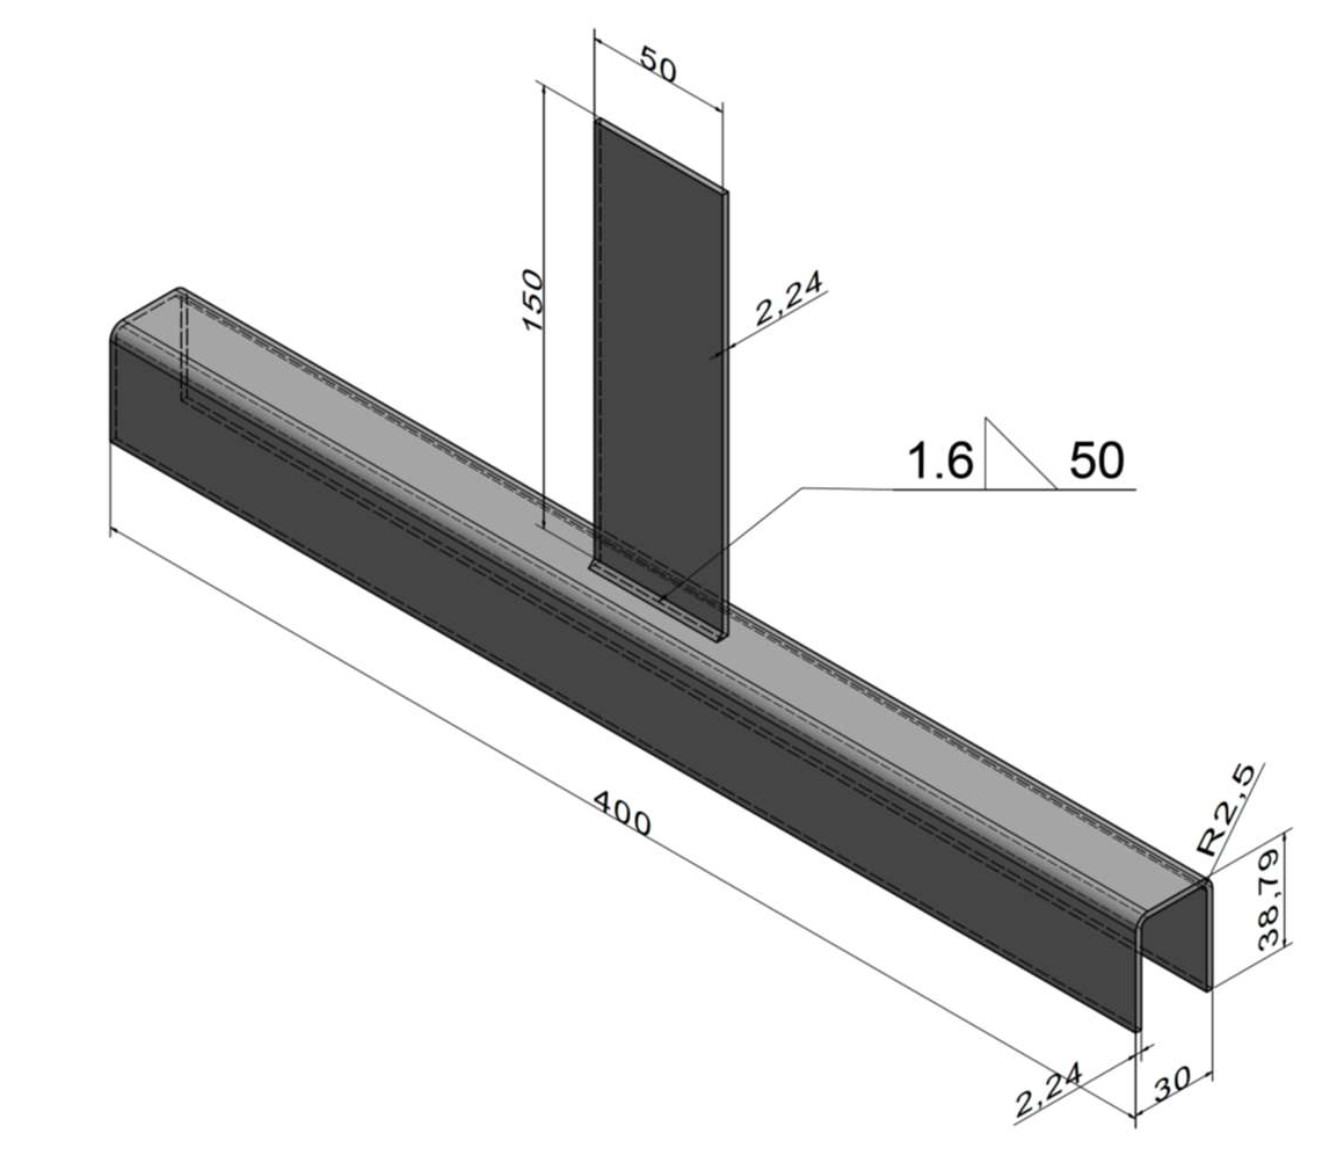
\includegraphics[width = 0.7\textwidth]{media/ditr.png}
    \caption{Συγκολλητή κατασκευή προς μελέτη.}
    \label{fig: ditr}
\end{figure}

Τα πειραματικά δεδομένα που έχουν δοθεί είναι για λόγο $R = 0$. Παρακάτω παρουσιάζονται τα δεδομένα για τον τύπο αστοχίας που φαίνεται στο \ref{fig:astoxia}. Όπως αναφέρθηκε και προηγουμένως, τα υπόλοιπα δύο δοκίμια και τα αποτελέσματα τους δεν λήφθηκαν υπόψη.
\par Για κάθε μία από τις μεθόδους, θα υπολογίζεται το εύρος τάσης για το κάθε δοκίμιο που ελέγχθηκε. Έπειτα, το έυρος αυτό θα συγκρίνεται με την αντίστοιχη καμπύλη διάρκειας ζωής σύμφωνα με τον οδηγό. Τα ζεύγη $(\Delta \sigma, N)$ που θα προκύπτουν θα αναφέρονται σε πιθανότητα επιβίωσης $50\%$. Επομένως, είναι αναγκαία και η μετατροπή σε πιθανότητα $97.7\%$ ώστε να μπορεί να γίνει η σύγκριση σύμφωνα με τον οδηγό IIW.

%pinakas dokimiws
\begin{table}[H]
    \centering
    \begin{tabular}{|c|c|c|c|}
        \hline
        \rowcolor{Dandelion}
        Spec No. & $F_m\; [kN]$ & $F_a\; [kN]$ & $N$\\
        \hline
        DI-01 & 28,2 & 27,9 & 89.000\\ \hline
        DI-02 & 37,6 & 37,3 & 29.000\\ \hline
        DI-03 & 34,2 & 33,9 & 41.000\\ \hline
        DI-04 & 31,2 & 30,9 & 73.000\\ \hline
        DI-05 & 40,2 & 39,9 & 23.000\\ \hline
        DI-06 & 22,1 & 22,0 & 190.000\\ \hline
        DI-08 & 18,1 & 18,0 & 603.000\\ \hline
        DI-09 & 20,1 & 20,0 & 453.000\\ \hline
        DI-10 & 21,1 & 21,0 & 575.000\\ \hline
        DI-11 & 26,2 & 26,0 & 167.000\\ \hline
        DI-12 & 16,5 & 16,4 & 1.470.000\\ \hline
        DI-13 & 23,2 & 23,0 & 335.000\\ \hline
        DI-15 & 24,2 & 24,0 & 246.000\\ \hline
    \end{tabular}
    \caption{Πειραματικά δεδομένα δοκιμής κόπωσης στη συγκολλητή κατασκευή.}
    \label{tab:spec}
\end{table}
%morfh astoxias A

\begin{figure}[H]
    \centering
    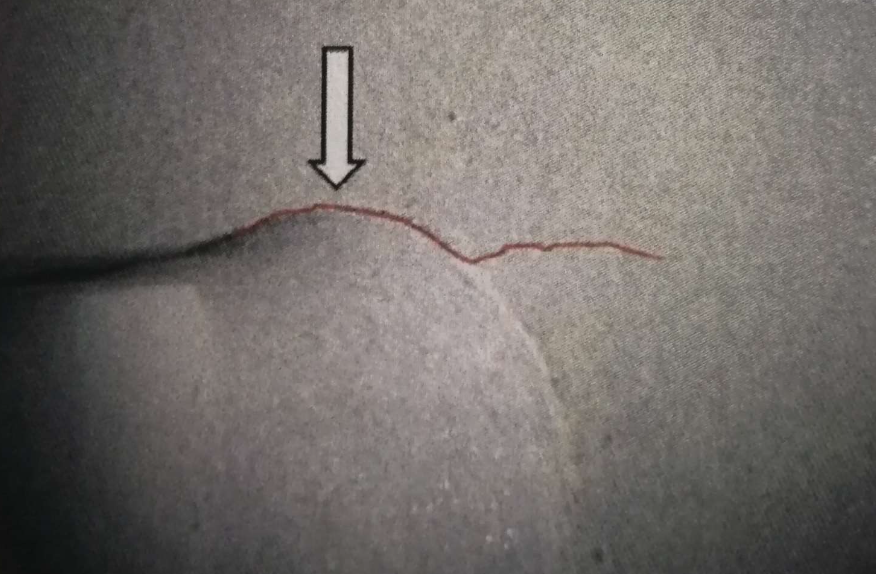
\includegraphics[width=0.5\linewidth]{media/astoxia.png}
    \caption{Μορφή αστοχίας πλειοψηφίας δοκιμίων.}
    \label{fig:astoxia}
\end{figure}

\subsection{Στατιστική ανάλυση}
Για τη δημιουργία της καμπύλης $97.7\%$ θα πρέπει να υπολογιστεί η τυπική απόκλιση $s$. Ορίζοντας ως:
\begin{align}
    \hat{y} &= log_{10} N\\
    \hat{x} &= log_{10} \Delta \sigma
\end{align}

Σύμφωνα με τους πίνακες της κανονικής κατανομής για να μετατραπούν τα σημεία στη ζητούμενη πιθανότητα αρκεί:
\begin{equation}
    \hat{y}_{97.7\%} = \hat{y}_{50\%} - 2.27s
\end{equation}

Από τα σημεία υπολογίζονται, κάθε φορά, οι συντελεστές $\alpha, \beta$ ως:
\begin{align}
    \beta &= \frac{\sum xy - \frac{\sum x \sum y}{n}}{\sum x^2 -n\overline{x}^2}\\
    \alpha &= \frac{\sum y}{n} - b\frac{\sum x}{n}
\end{align} 

Έπειτα, υπολογίζεται η τυπική απόκλιση ως:
\begin{equation}
    s = \sqrt{\frac{\sum (y(\overline{x}) - \overline{y})^2}{n}}
\end{equation}




\section{Υπολογισμοί συγκόλλησης}

\subsection{Συντελεστές διόρθωσης} 
Οι συντελεστές διόρθωσης που εφαρμόστηκαν τόσο στη μέθοδο της ονομαστικής τάσης, όσο και στη κατασκευαστική τάση, έχουν να κάνουν με τη διόρθωση της τυποποιημένης καμπύλης για την αξιολόγηση της διάρκειας ζωής. Οι συντελεστές αυτοί αφορούν τον λόγο φόρτισης $R$ και το πάχος του ελάσματος $t$ προς συγκόλληση.
\par Ο συντελεστής λόγου φόρτισης δηλώνει πως:
\begin{equation}
    f(R) = -0.4\cdot R + 1.2,\; \text{for} -1\le R \le 0.5
\end{equation}
Αντίστοιχα, ο συντελεστής πάχους υπολογίζεται για:
\begin{equation}
    t_{eff} = max\{0.5\cdot L, t\},
\end{equation}
καθώς ισχύει ότι $L/t>2$. Τελικά, ο συντελεστής δίνεται ως:

\begin{equation}
    f(t) = \bigg(\frac{t_{ref}}{t_{eff}}\bigg)^n
\end{equation}

Προκύπτει λοιπόν ότι ο συνολικός συντελεστής $f(tot) = f(R)\cdot f(t) = 1.2$. Έτσι, η κλάση (δηλαδή το όριο αντοχής στους στους $2\cdot 10^6$ κύκλους φόρτισης) μετατοπίζεται προς τα πάνω στα αντίστοιχα διαγράμματα εύρους τάσης - διάρκειας ζωής:
\begin{equation}
    FAT_{assess} = f(tot) \cdot FAT_{ref}
\end{equation}



\subsection{Μέθοδος Ονομαστικής Τάσης}
Για τη μέθοδο της ονομαστικής τάσης, αρκεί ο υπολογισμός των ονομαστικών τάσεων από τις φορτίσεις της κατασκευής. Αυτές σύμφωνα με τον οδηγό υπολογίζονται ως:
\begin{equation}
    \sigma = \frac{F}{A_w}
\end{equation}
Στη περίπτωση της δύναμης κάθετα προς τη ραφή της συγκόλλησης ο οδηγός IIW αναφέρει ότι η διατομή που χρησιμοποιείται εξαρτάται από μήκος της συγκόλλησης και το πάχος της ως:
\begin{equation}
    A_w = l\cdot a_w
\end{equation}
Στη περίπτωση προς μελέτη ωστόσο, η ραφή είναι παράλληλη προς την διεύθυνση της δύναμης. Έτσι, σαν διατομή συγκόλλησης επιλέγεται η διατομή της βάσης της συγκόλλησης (του κύριου τεμαχίου σε σχήμα Π). Τέλος, υπολογίζεται το εύρος τάσης για κάθε διαφορετικό δοκίμιο ως:
\begin{equation}
    \Delta \sigma = 2\cdot \frac{F_a}{A_w}
\end{equation}

Έχοντας υπολογίσει λοιπόν, τα σημεία $(\Delta \sigma, N)$, τα οποία εκφράζουν την $50\%$ πιθανότητα επιβίωσης, εξάγονται τα σημεία και για την $97.7\%$ πιθανότητα. Αυτό γίνεται, έτσι ώστε να συγκρίνονται όμοιες καμπύλες διάρκειας ζωής μεταξύ τους. Οι καμπύλες για την αξιολόγηση διάρκειας ζωής FAT εκφράζουν και αυτές την $97.7\%$ σύμφωνα με τον IIW. Ο οδηγός αναφέρει ότι για την ανάλυση σε κόπωση με τη μέθοδο της ονομαστικής τάσης, πρέπει η καμπύλη διάρκειας ζωής να συγκριθεί με κάποια από τις τυποποιημένες καμπύλες FAT του οδηγού. Αρκεί λοιπόν, να επιλεχθεί η κατάλληλη κλάση FAT ώστε να εκτιμηθεί η διάρκεια ζωής της κατασκευής.
\par Σύμφωνα με τον οδηγό, η κλάση τυποποιημένης καμπύλης διάρκειας ζωής που βρίσκεται πιο κοντά στη παρόν περίπτωση είναι η \textit{FAT 71}. Το μήκος της συγκόλλησης είναι $50\; mm$ και έτσι, η επιλεγμένη κλάση προέκυψε από τον παρακάτω πίνακα.
\begin{figure}[H]
    \centering
    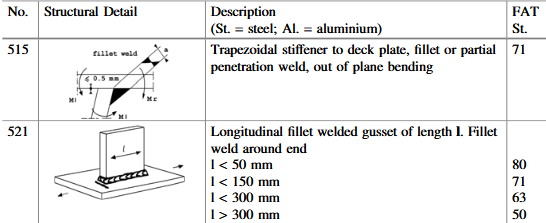
\includegraphics[width = 0.5\linewidth]{media/fatnom.png}
    \caption{Κλάσεις τυποποιημένων καμπύλων αξιολόγησης διάρκειας ζωής, FAT, για διάφορες κατασκευαστικές λεπτομέρειες, σύμφωνα με τη μέθοδο της ονομαστικής τάσης και του οδηγού IIW.}
\end{figure}


\subsection{Μέθοδος Κατασκευαστικής Τάσης}
Σκοπός της μεθόδου της κατασκευαστικής τάσης είναι να υπολογιστεί η τάση στο πόδι της συγκόλλησης, εκεί που αναμένεται η αστοχία. Αυτό γίνεται με διάφορους τρόπους. Στη παρόν μελέτη επιλέχθηκε η μέθοδος του extrapolation. Σύμφωνα με αυτήν, υπολογίζεται η κατασκευαστική τάση σε μερικά σημεία ενδιαφέροντος κοντά στο πόδι της συγκόλλησης και έπειτα μέσω αυτών καταλήγει κανείς στην κατασκευαστική τάση.
\par Προφανώς, για να επιτευχθεί αυτό έγκειται η ανάγκη της χρήσης της μεθόδου των ΠΣ. Επομένως, πρέπει να δημιουργηθεί το αντίστοιχο μοντλέλο ΠΣ προς επίλυση. Σύμφωνα με τους κανονισμούς του οδηγού για τη μοντελοποίηση ΠΣ, επιλέγονται δισδιάστατα στοιχεία κελύφους για τα ελάσματα που έχουν συγκολληθεί. Τα στοιχεία αυτά επιβάλλεται να είναι δευτέρου βαθμού για μεγαλύτερη ακρίβεια. Σχετικά με το πλέγμα, για να υπολογιστεί η κατασκευαστική τάση πρέπει να δημιουργηθεί κατάλληλο πλέγμα στο μοντέλο. Πριν δημιουργηθεί αυτό είναι μεγάλης σημαντικότητας η επιλογή μερικών παραμέτρων για τη συγκόλληση.
\par Αρχικά, επιλέγεται ο τύπος hot-spot. Οι δύο διαφορετικοί τύποι είναι οι a, b, όπου ξεχωρίζουν σύμφωνα με τον οδηγό από το \ref{fig:hstype}. Για το συγκεκριμένο, υπό μελέτη δοκίμιο, επιλέγεται ο τύπος a.
\begin{figure}[H]
    \centering
    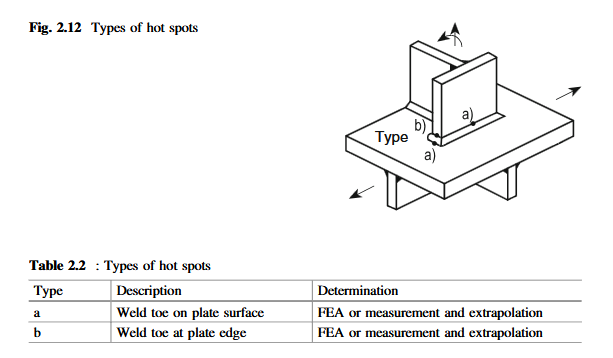
\includegraphics[width = 0.5\linewidth]{media/hstype.png}
    \caption{Τύποι hot-spot σε συγκολλητές κατασκευές.}
    \label{fig:hstype}
\end{figure}
\par Έπειτα, επιλέγεται η πύκνωση του πλέγματος. Ανάλογα με αυτήν επιλέγονται και τα σημεία μέτρησης τάσης για τη μέθοδο του extrapolation. Εδώ, επιλέγονται δύο σημεία σύμφωνα με τη μοντελοποίηση με πυκνό πλέγμα, όπου τα στοιχεία κελύφους δεν πρέπει να είναι μεγαλύτερα από $0.4 t \times t$. Τα σημεία για το extrapolation βρίσκονται σε αποστάσεις $0.4t$ και $1.0t$, όπως φαίνεται παρακάτω.

\begin{figure}[H]
    \centering
    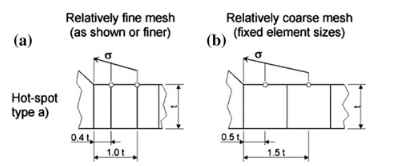
\includegraphics[width = 0.5\linewidth]{media/plegmahs.png}
    \caption{Σημεία για extrapolation σύμφωνα με τη μέθοδο της κατασκευαστικής τάσης.}
    \label{fig:plegmahs}
\end{figure}

Από τα σημεία αυτά, υπολογίζεται η κατασκευαστική τάση ως:
\begin{equation}
    \sigma_{hs} = 1.67 \sigma_{0.4t} -0.67 \sigma_{1.0t}
\end{equation}
Επομένως, πρέπει το πλέγμα να φέρει τα αντίστοιχα σημεία κοντά στο πόδι της συγκόλλησης για τον υπολογισμό των τάσων $\sigma_{0.4t}, \sigma_{1.0t}$.
\par Τέλος, η συγκόλληση μοντελοποιείται επίσης με στοιχεία κελύφους, πάχους όσο το πάχος της συγκόλλησης και γεωμετρικά στη μέση επιφάνεια της συγκόλλησης. Η επιφάνεια αυτή εκτείνεται έως ότου να τμήσει τα δύο τεμάχια προς συγκόλληση. Οι οδηγίες αυτές έχουν δοθεί προφανώς από τον οδηγό και η διαδικασία γίνεται πιο εύκολα κατανοητή από το \ref{fig:sygkpl}. Το τελικό πλέγμα προς επίλυση φαίνεται στο \ref{fig:grid}.

\begin{figure}[H]
    \centering
    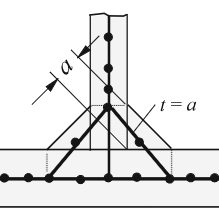
\includegraphics[width = 0.2\linewidth]{media/sygkpl.png}
    \caption{Μοντελοποίηση συγκόλλησης σύμφωνα με τον οδηγό IIW.}
    \label{fig:sygkpl}
\end{figure}

\begin{figure}[H]
    \centering
    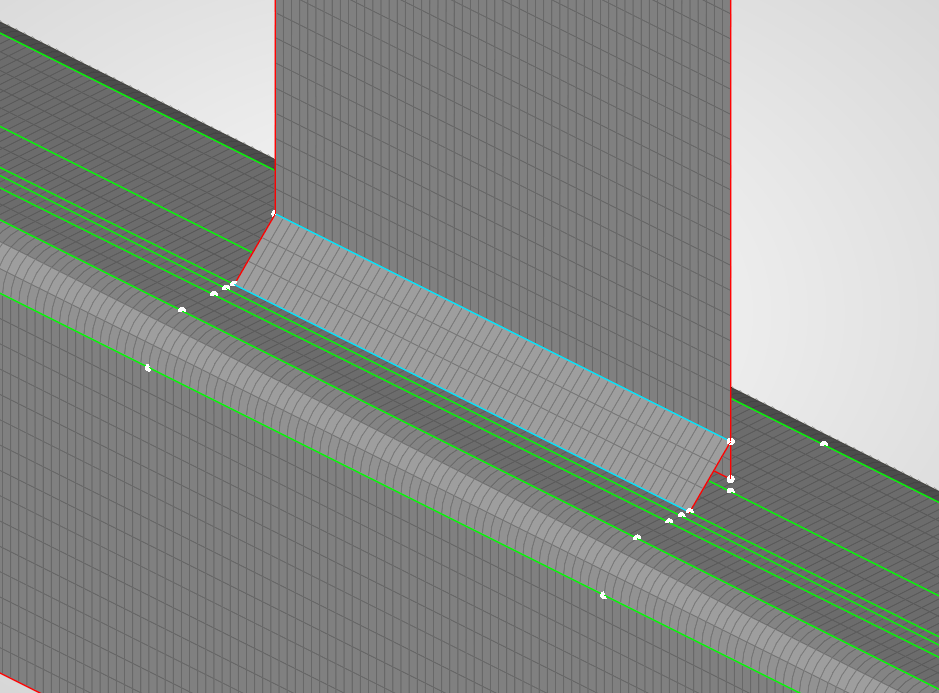
\includegraphics[width = 0.7\linewidth]{media/grid.png}
    \caption{Πλέγμα μοντέλου επίλυσης για τη μέθοδο της κατασκευαστικής τάσης σύμφωνα με τις οδηγίες του IIW.}
    \label{fig:grid}
\end{figure}

Εν τέλει, υπολογίζονται για άλλη μία φορά τα εύρη τάσης ως:
\begin{equation}
    \Delta \sigma_{hs} = \sigma_{hs,max} - \sigma_{hs,min},
\end{equation}
και μετατρέπονται πάλι στην αναγκαία πιθανότητα επιβίωσης για σύγκριση. Οι τάσεις που εξάγονται είναι οι μέγιστες κύριες στην άνω επιφάνεια μετρούμενες στη γωνία.
\par Όσο αναφορά την αξιολόγηση της διάρκειας ζωής, σύμφωνα με τον οδηγό, οι καμπύλες που χρησιμοποιούνται δίνονται από το \ref{fig:faths}. Εδώ, επιλέγεται η FAT 100 για αξιολόγηση, η οποία τροποποιείται πάλι με βάση τους συντελεστές διόρθωσης.
\begin{figure}[H]
    \centering
    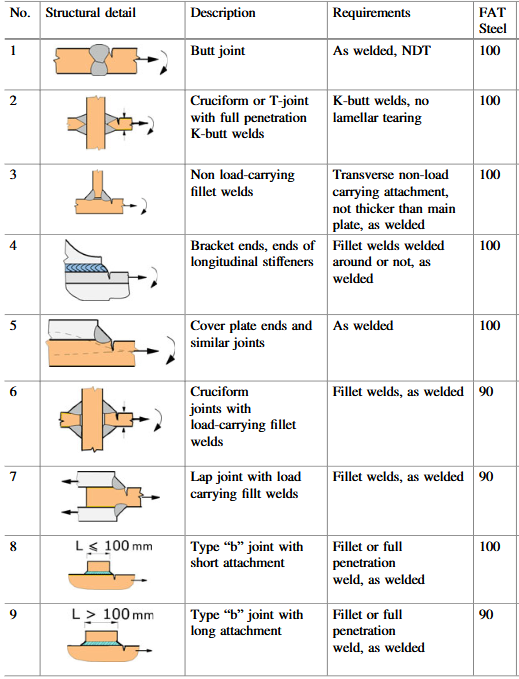
\includegraphics[width = 0.45\linewidth]{media/hsfat.png}
    \caption{Κλάσεις τυποποιημένων καμπύλων αξιολόγησης διάρκειας ζωής, FAT, για διάφορες κατασκευαστικές λεπτομέρειες, σύμφωνα με τη μέθοδο της κατασκευαστικής τάσης και του οδηγού IIW.}
    \label{fig:faths}
\end{figure}


\subsection{Μέθοδος Ενεργής Τάσης Εγκοπής}
Αναφορικά με την ενεργή τάση εγκοπής, αυτή ορίζεται ως η τάση στη ρίζα της συγκόλλησης. Λόγω της δυσκολίας υπολογισμού αυτής της τάσης, ο οδηγός ορίζει την ενεργή τάση εγκοπής για την αξιολόγηση της διάρκειας ζωής της συγκολλητής κατασκευής. 
\par Η τάση αυτή υπολογίζεται μέσω επίλυσης μοντέλου ΠΣ. Το μοντέλο αυτό έχει πολύ συγκεκριμένες προδιαγραφές. Ο οδηγός αναφέρει μεθόδους μοντελοποίησης για κατασκευές με πάχος μεγαλύτερου των 5 χιλιοστών. Κάτι τέτοιο, δεν αρμόζει στη παρόν μελέτη. Ωστόσο, πρόσφατες μελέτες έχουν κατά κάποιο τρόπο επεκτείνει τη μεθδολογία του οδηγού και σε κατασκευές με μικρότερα πάχη. Μια εξ αυτών αναγράφεται στην \cite{BAUMGARTNER2020105844}. Εδώ, αναφέρεται ότι για λεπτόπαχα ελάσματα πρέπει να χρησιμοποιείται ακτίνα καμπυλότητας $\rho = 0.05 \;mm$ για τη μοντελοποίηση της ρίζας και κλίση FAT $m=5$. Επίσης, σύμφωνα με την \cite{malik}, δίνεται η μορφή του μοντέλου ΠΣ και της ρίζας με διευρυμένο διάκενο προς την πλευρά αποκλειστικά του συνδεόμενου ελάσματος. Αναγράφεται επίσης, ότι η αξιολόγηση διάρκειας ζωής γίνεται σύμφωνα με το όριο FAT 630 για εξαγωγή αποτελεσμάτων μέγιστης κύριας τάσης.

\section{Αποτελέσματα Και Συζήτηση}

\listoffigures
\listoftables



\printbibliography
\end{document}